\section{Durchführung}
\label{sec:Durchführung}

Der Aufbau des Versuches beinhaltet drei Elemente; einem Laser (hier mit der 
Wellenlänge von $\lambda = 633 \unit{\nano\meter}$), einem Spalt mit einer 
Breite im $\unit{\micro\meter}$-Bereich und einem Photoelement, welches auf 
einem Schiebereiter um jeweils $25 \unit{\milli\meter}$ um den Mittelpunkt 
verschoben werden kann. Angeschlossen an ein Amperemeter, kann damit die 
Intensität in einem Bereich detektiert werden. Alle drei Elemente befinden 
sich auf einer Schiene. Der Abstand zwischen Laser und Detektor wird als 
Länge $L$ betitelt sowie die Abweichung vom Ursprungsstrahl als Winkel 
$\varphi$.
\begin{figure}[H]
    \centering
    \begin{minipage}{0.45\textwidth}
        \label{fig:f2}
        \centering
        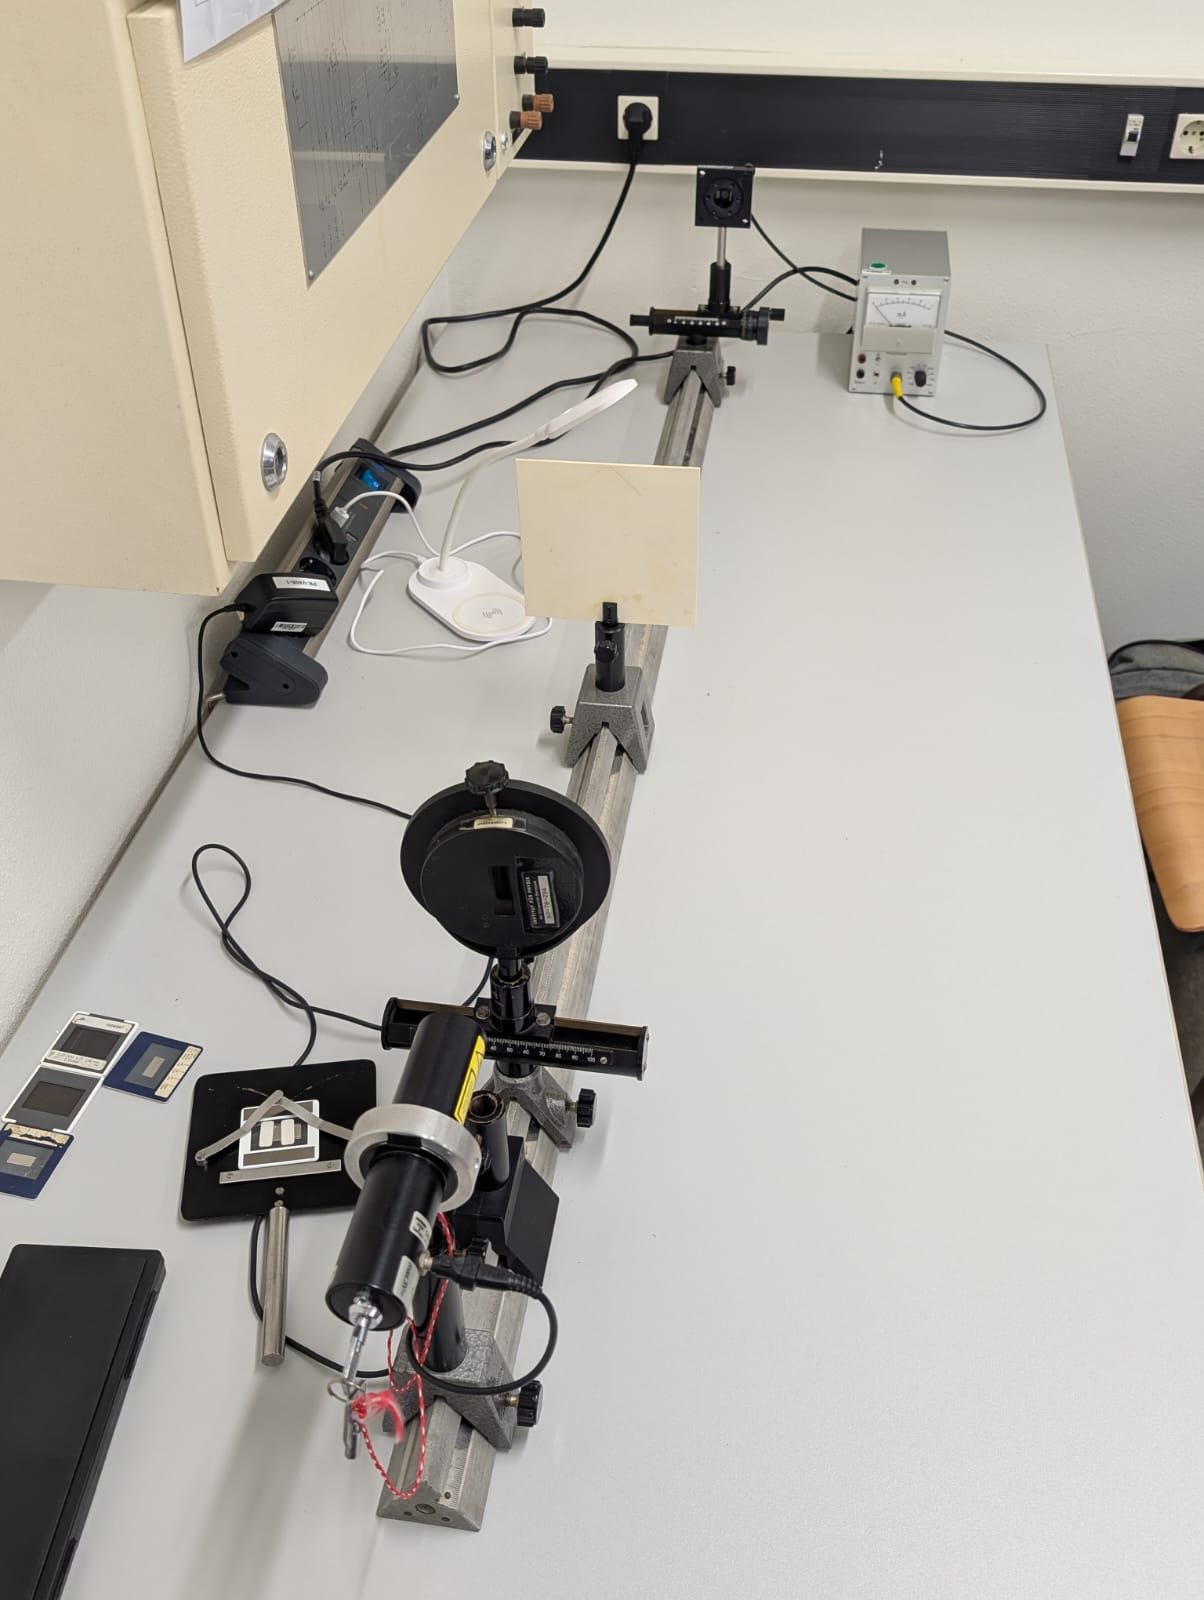
\includegraphics[width=\textwidth]{Bilder/A1.jpg}
        \caption{Aufbau (vom Laser aus).}
    \end{minipage}
    \hfill
    \begin{minipage}{0.53\textwidth}
        \label{fig:f3}
        \centering
        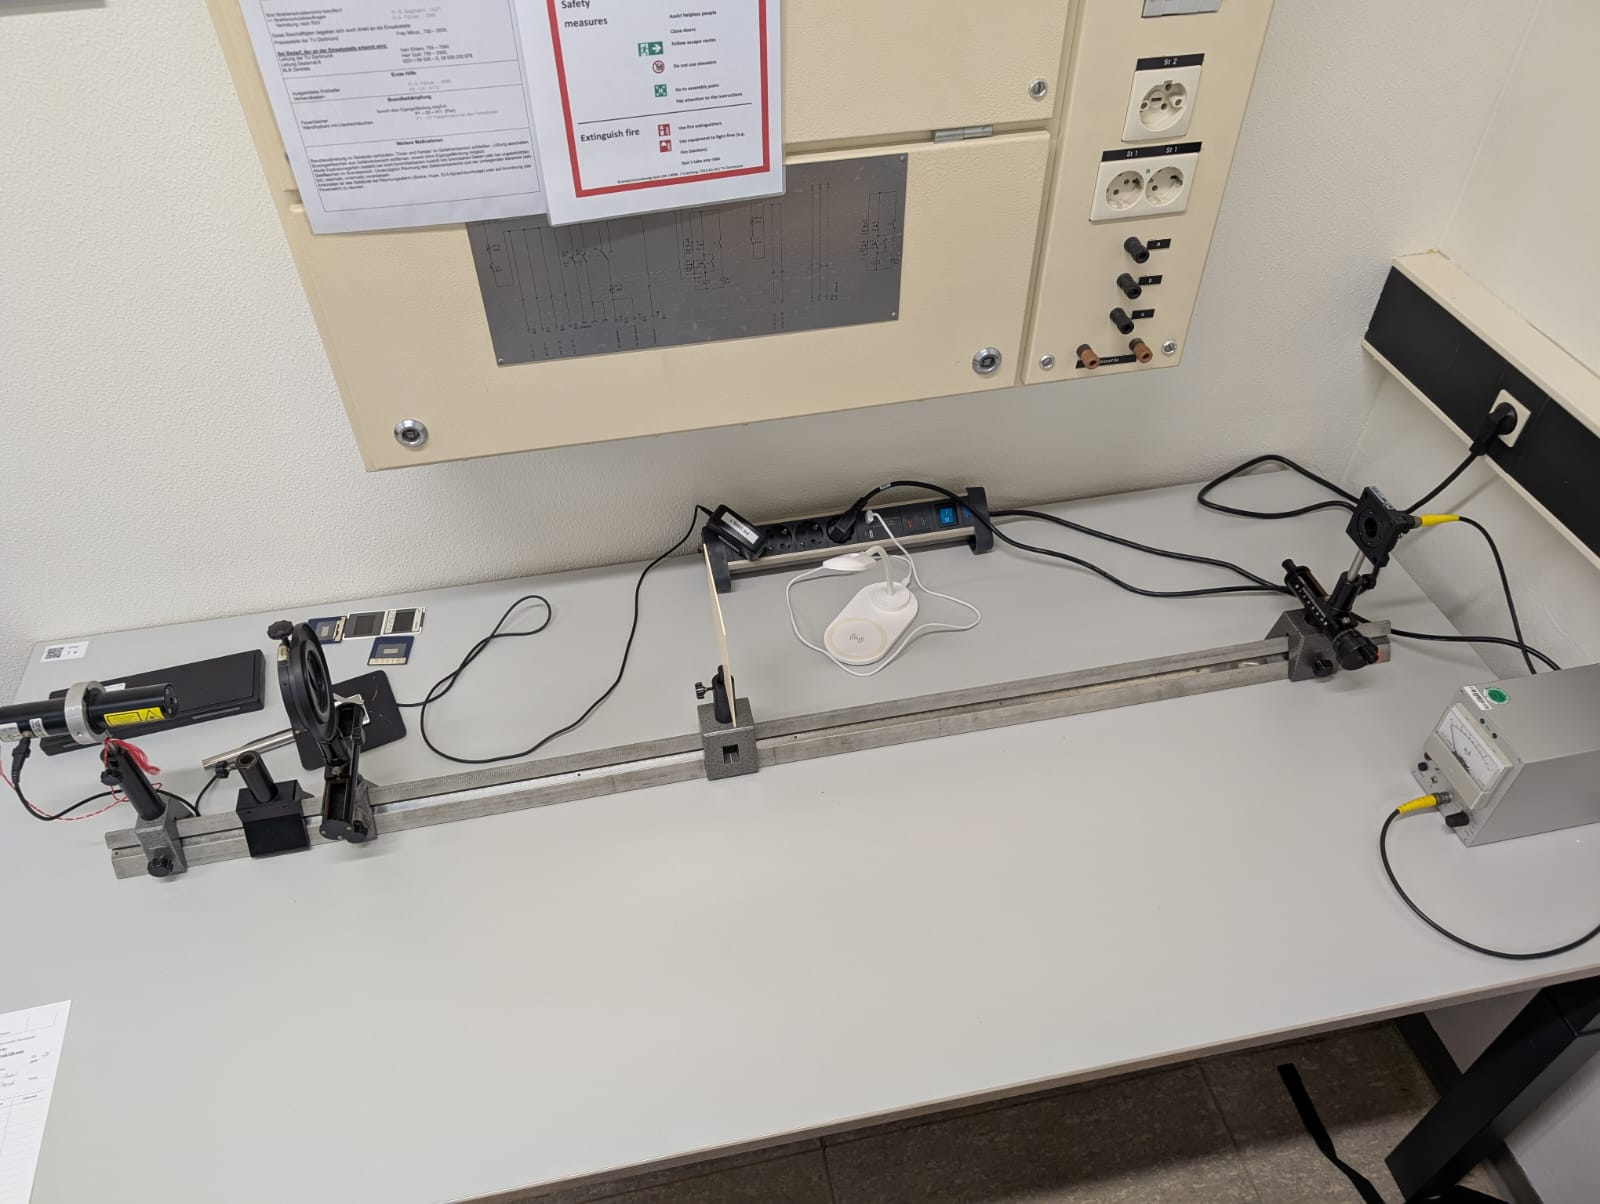
\includegraphics[width=\textwidth]{Bilder/A2.jpg}
        \caption{Aufbau (von vorne).}
    \end{minipage}
\end{figure}
\noindent Um Messungsfehler seitens des Amperemeters zu minimieren, wird der Raum 
abgedunkelt und eine Nullmessung durchgeführt. Diese dient im späteren Verlauf 
dem Zweck mögliche Anfangsresonanzen/Anfangswerte im Gerät herauszufiltern.
Nach den präventativen Vorkehrungen startet das tatsächliche Experiment und 
der Laser wird aktiviert. Angefangen ganz links des Schiebereiters wird der 
gemessene Strom am Amperemeter dokumentiert. Der Mittelpunkt sei bei $\zeta_0$
(siehe \autoref{fig:f2}).
Messungen im Bereich oberhalb dieses Mittelpunkts seien im Folgenden als 
negative Länge definiert. Jegliche Werte unterhalb des Mittelpunkts seien 
regulär positiv.
\begin{figure}[H]
    \centering
        \centering
        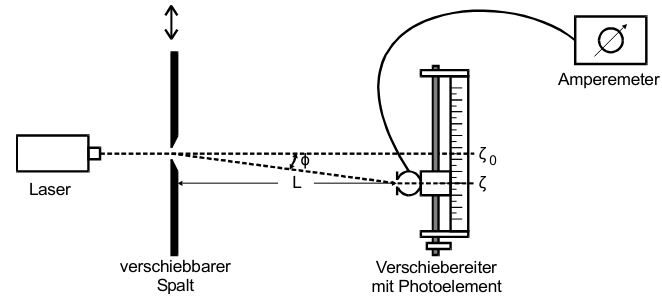
\includegraphics[width=1.0\textwidth]{Bilder/aufbau.png}
        \caption{Aufbau des Versuches. \cite{anleitung3}}
    \hfill
    \label{fig:f2}
\end{figure}
\noindent Bei $-25 \unit{\milli\meter}$ bis $-11 \unit{\milli\meter}$ wird die 
Intensität am Amperemeter in $1 \unit{\milli\meter}$-Abständen gemessen.
Im Bereich von $-10.5 \unit{\milli\meter}$ bis $10 \unit{\milli\meter}$ wird
in $0.5 \unit{\milli\meter}$-Schritten gemessen und anschließend bis zum Ende 
des Reiters wieder in $1 \unit{\milli\meter}$-Schritten. In dem mittleren Bereich 
wird ein anderer Messabstand gewählt, um das Hauptmaximum besser dokumentieren 
zu können. Bei dem Doppelspalt wird im Bereich von $-25 \unit{\milli\meter}$
bis $-10 \unit{\milli\meter}$ und von $-10 \unit{\milli\meter}$ bis 
$25 \unit{\milli\meter}$ bereits in $0.5 \unit{\milli\meter}$-Schritten gemessen.
Im Bereich dazwischen wird mit $0.25 \unit{\milli\meter}$-Schritten gemessen.
